\documentclass[11pt]{article}
% force pdfLaTeX on arXiv (needed with PNG graphics); skip under XeTeX/LuaTeX
\ifdefined\pdfoutput\ifdefined\XeTeXversion\else\pdfoutput=1\fi\fi
\usepackage[margin=1in]{geometry}
\usepackage{graphicx}
\usepackage{booktabs}
\usepackage{amsmath}
\usepackage{xcolor}
\usepackage{hyperref}
\usepackage{caption}
\usepackage{float}
\hypersetup{colorlinks=true, linkcolor=teal, urlcolor=teal, citecolor=teal}
\definecolor{win}{HTML}{2A9D8F}
\definecolor{teach}{HTML}{E76F51}

\title{\textbf{Distilling an LLM Diagram-Curation Pipeline\\into Local Classifiers}\\[4pt]
\large A practical study on one MacBook: data creation, a model ladder,\\
measurements, and a production decision}
\author{Adnan Abbasi}
\date{July 2026}

\begin{document}
\maketitle

\begin{abstract}
\noindent
A frozen SigLIP2 image encoder with a logistic-regression head classifies
figure crops as diagram / not-diagram at \textbf{86.0\% against hand-verified
truth} (95\% CI [81.5, 90.5]), beating the vision-LLM pipeline that
\emph{generated its training labels} by \textbf{10.5 points} (75.5\%; McNemar
$p=0.0005$), at \textbf{$\sim$52\,ms/crop on a laptop GPU} versus 4--17\,s per
LLM call --- offline, deterministic, at zero marginal cost. Zero-shot SigLIP2
(no training) also beats the LLM (83.5\%, statistically tied with the trained
probe). The complex options lost: an end-to-end fine-tune (71.5\%) and MLP
heads (78.0\%) overfit the teacher's $\sim$25\% label noise, and an
off-the-shelf document layout detector for the page gate scored 61.7\% while
running 100$\times$ slower. We release the pipeline, the 2{,}000-diagram
dataset, and all code. The central methodological lesson: under LLM
distillation with noisy labels, validate against a hand-verified gold set or
you will ship the wrong model --- silver validation ranked the worst-generalizing
model first.
\end{abstract}

\section{Problem and contribution}
We curate a dataset of \emph{proper technical diagrams} (block diagrams,
schematics, flowcharts, architectures --- not data plots, photos, or fragments)
from arXiv papers in six engineering fields, each image paired with a detailed
label. Our production pipeline (v2) routes every page and every extracted crop
through paid vision-LLM calls for two \emph{classification} decisions --- a
page gate (``does this page contain a diagram?'') and a crop gate (``is this a
proper diagram?'') --- plus a genuinely \emph{generative} labeling step. This
paper asks whether the two classification gates can be replaced by local
models on a laptop at equal-or-better accuracy and far better speed. The
answer is yes, decisively, and the winning model is almost the simplest thing
one can build.

\section{How the data was created}
Six arXiv field queries yielded 1{,}183 downloaded papers. A cheap screening
model (\texttt{seed-1.6-flash}) proposes candidate diagram pages; a stronger
model (\texttt{xiaomi/mimo-v2.5}) confirms; Mistral OCR extracts figure crops
from confirmed pages; and \texttt{mimo-v2.5} classifies-and-labels each crop
with strict rejection of plots, photos, fragments, and blanks. Free local
pre-filters skip zero-graphics pages and tiny/blank crops. The run produced
\textbf{2{,}000 accepted diagrams}, 3{,}868 rejected crops (with reasons), and
12{,}266 LLM-judged pages, for \$20.36 total, fully resumable (it survived
credit exhaustion and two hard shutdowns without loss). Figure~\ref{fig:funnel}
shows the funnel.

Because every decision was journaled to SQLite, the classifier training sets
are a byproduct: crops with 4-class silver labels (diagram / data\_plot /
photo / fragment), pages with binary silver labels, and a paper-level
70/15/15 split (no paper crosses splits).

\begin{figure}[H]\centering
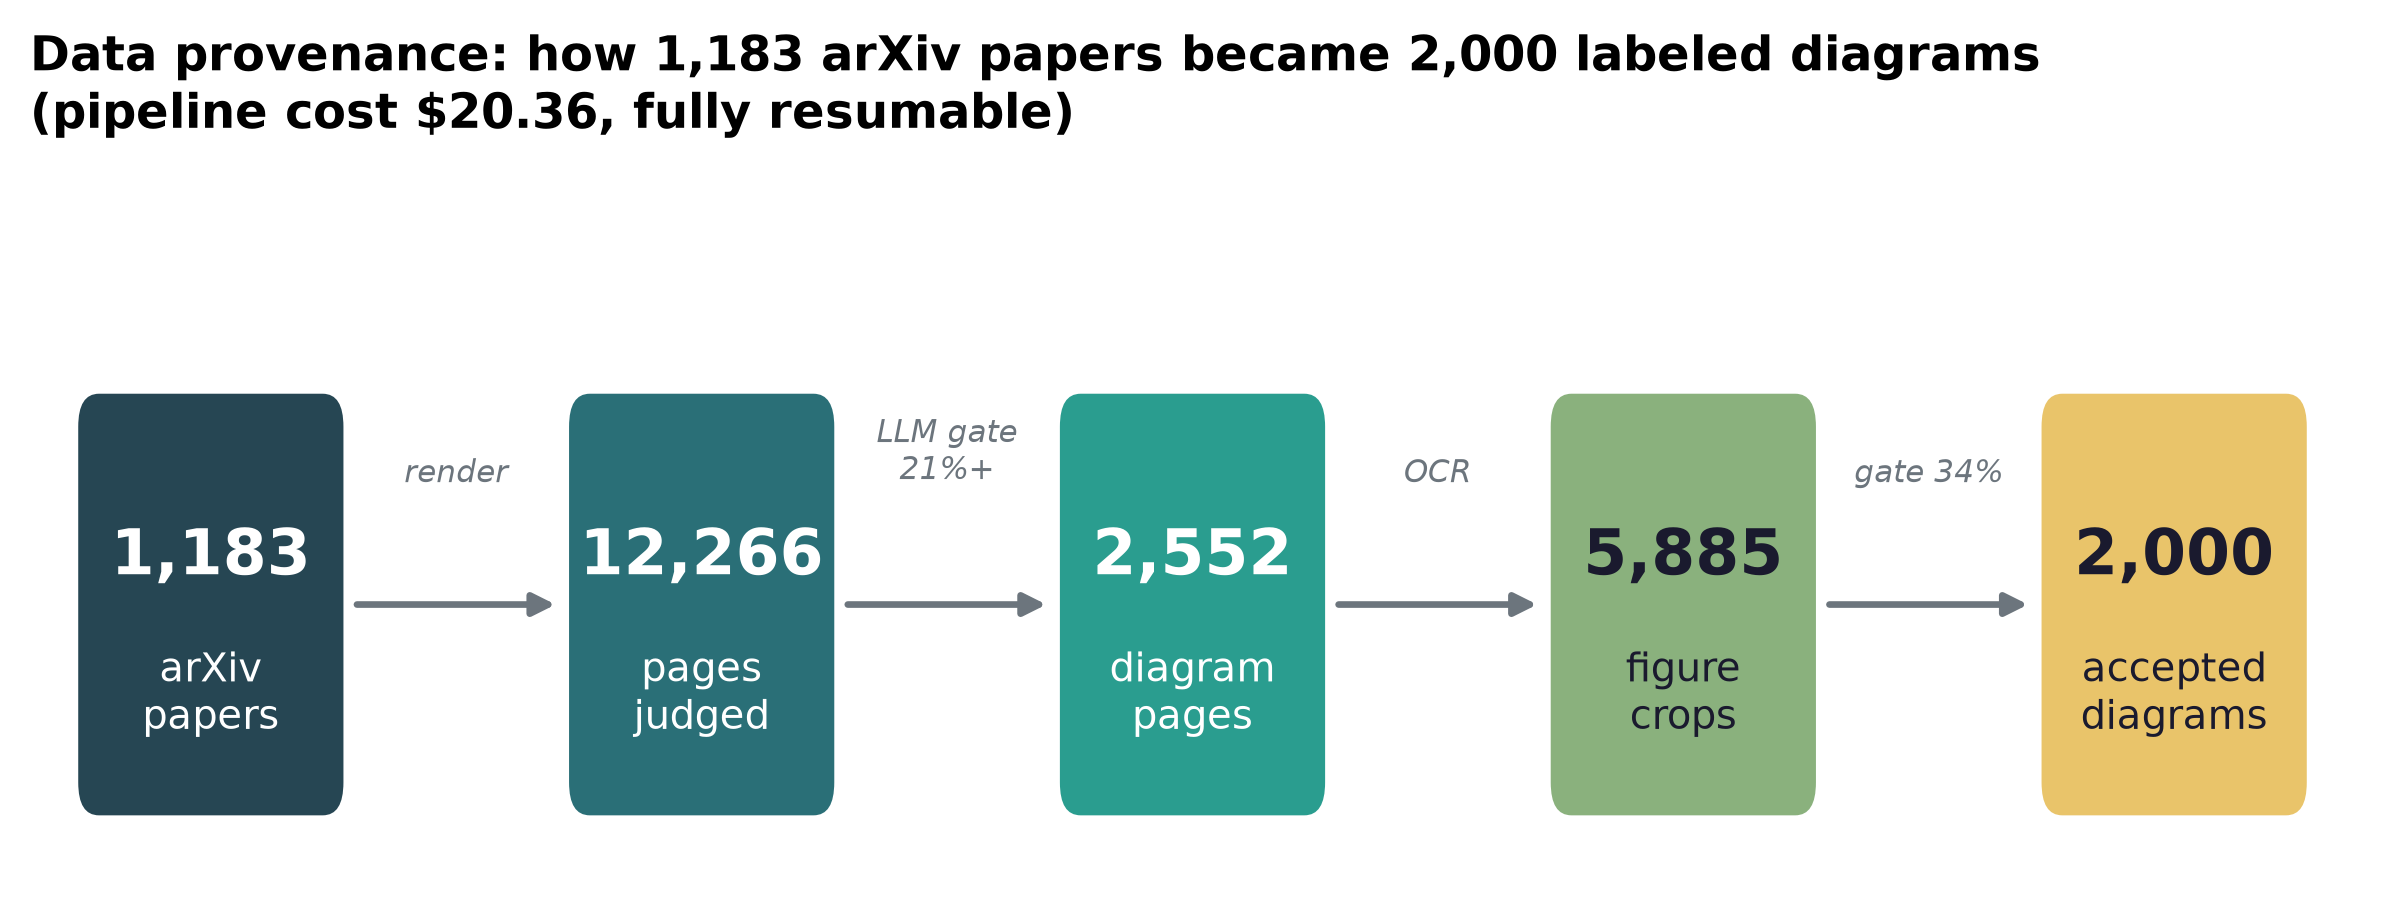
\includegraphics[width=0.86\textwidth]{figures/fig4_data_funnel.png}
\caption{Data provenance. The pipeline is the ``teacher''; its decisions become
the students' training labels.}
\label{fig:funnel}
\end{figure}

\section{Gold labels: the measurement instrument}
Silver labels are LLM opinions. All headline numbers use \textbf{gold} labels:
200 test-split crops and 120 test-split pages, labeled \emph{blind} against a
versioned rubric by two independent annotators (Claude Sonnet agents with no
access to model outputs), disagreements adjudicated by the lead. Inter-rater
reliability was $\kappa=0.925$ (crops, 4-class) and $0.940$ (binary) --- a
sound instrument. Critically, \textbf{the LLM teacher itself scores only
75.5\% on gold crops and 80.0\% on gold pages}: it systematically over-accepts
annotated plots and photos (precision 0.675 / 0.600). A student can therefore
beat its teacher, and ``agreement with the LLM'' is not the same as accuracy.

\section{The model ladder and results}
We ran approaches in ascending complexity, each justified only if it beat the
previous. Table~\ref{tab:gold} gives the gold-test headline.

\begin{table}[H]\centering
\caption{Crop gate, binary accept/reject vs.\ hand-verified gold ($n=200$).}
\label{tab:gold}
\begin{tabular}{lccccc}
\toprule
Model & Gold acc & 95\% CI & F1 & Prec. & Rec. \\
\midrule
\textbf{\textcolor{win}{SigLIP2 + logreg}} & \textbf{0.860} & [0.815, 0.905] & 0.854 & 0.812 & 0.901 \\
Zero-shot SigLIP2 & 0.835 & [0.785, 0.885] & 0.837 & 0.759 & 0.934 \\
SigLIP2 + MLP & 0.780 & [0.725, 0.835] & 0.796 & 0.688 & 0.945 \\
DINOv2 + MLP & 0.765 & [0.710, 0.825] & 0.773 & 0.690 & 0.879 \\
\textcolor{teach}{LLM teacher (mimo-v2.5)} & 0.755 & [0.700, 0.815] & 0.768 & 0.675 & 0.890 \\
MobileCLIP-S0 + MLP & 0.750 & [0.695, 0.810] & 0.766 & 0.667 & 0.901 \\
DINOv3 + MLP & 0.735 & [0.675, 0.795] & 0.762 & 0.644 & 0.934 \\
EfficientNet-B0 fine-tune & 0.715 & [0.650, 0.775] & 0.695 & 0.677 & 0.714 \\
Heuristics (GBT) & 0.625 & [0.555, 0.695] & 0.678 & 0.556 & 0.868 \\
\bottomrule
\end{tabular}
\end{table}

\begin{figure}[H]\centering
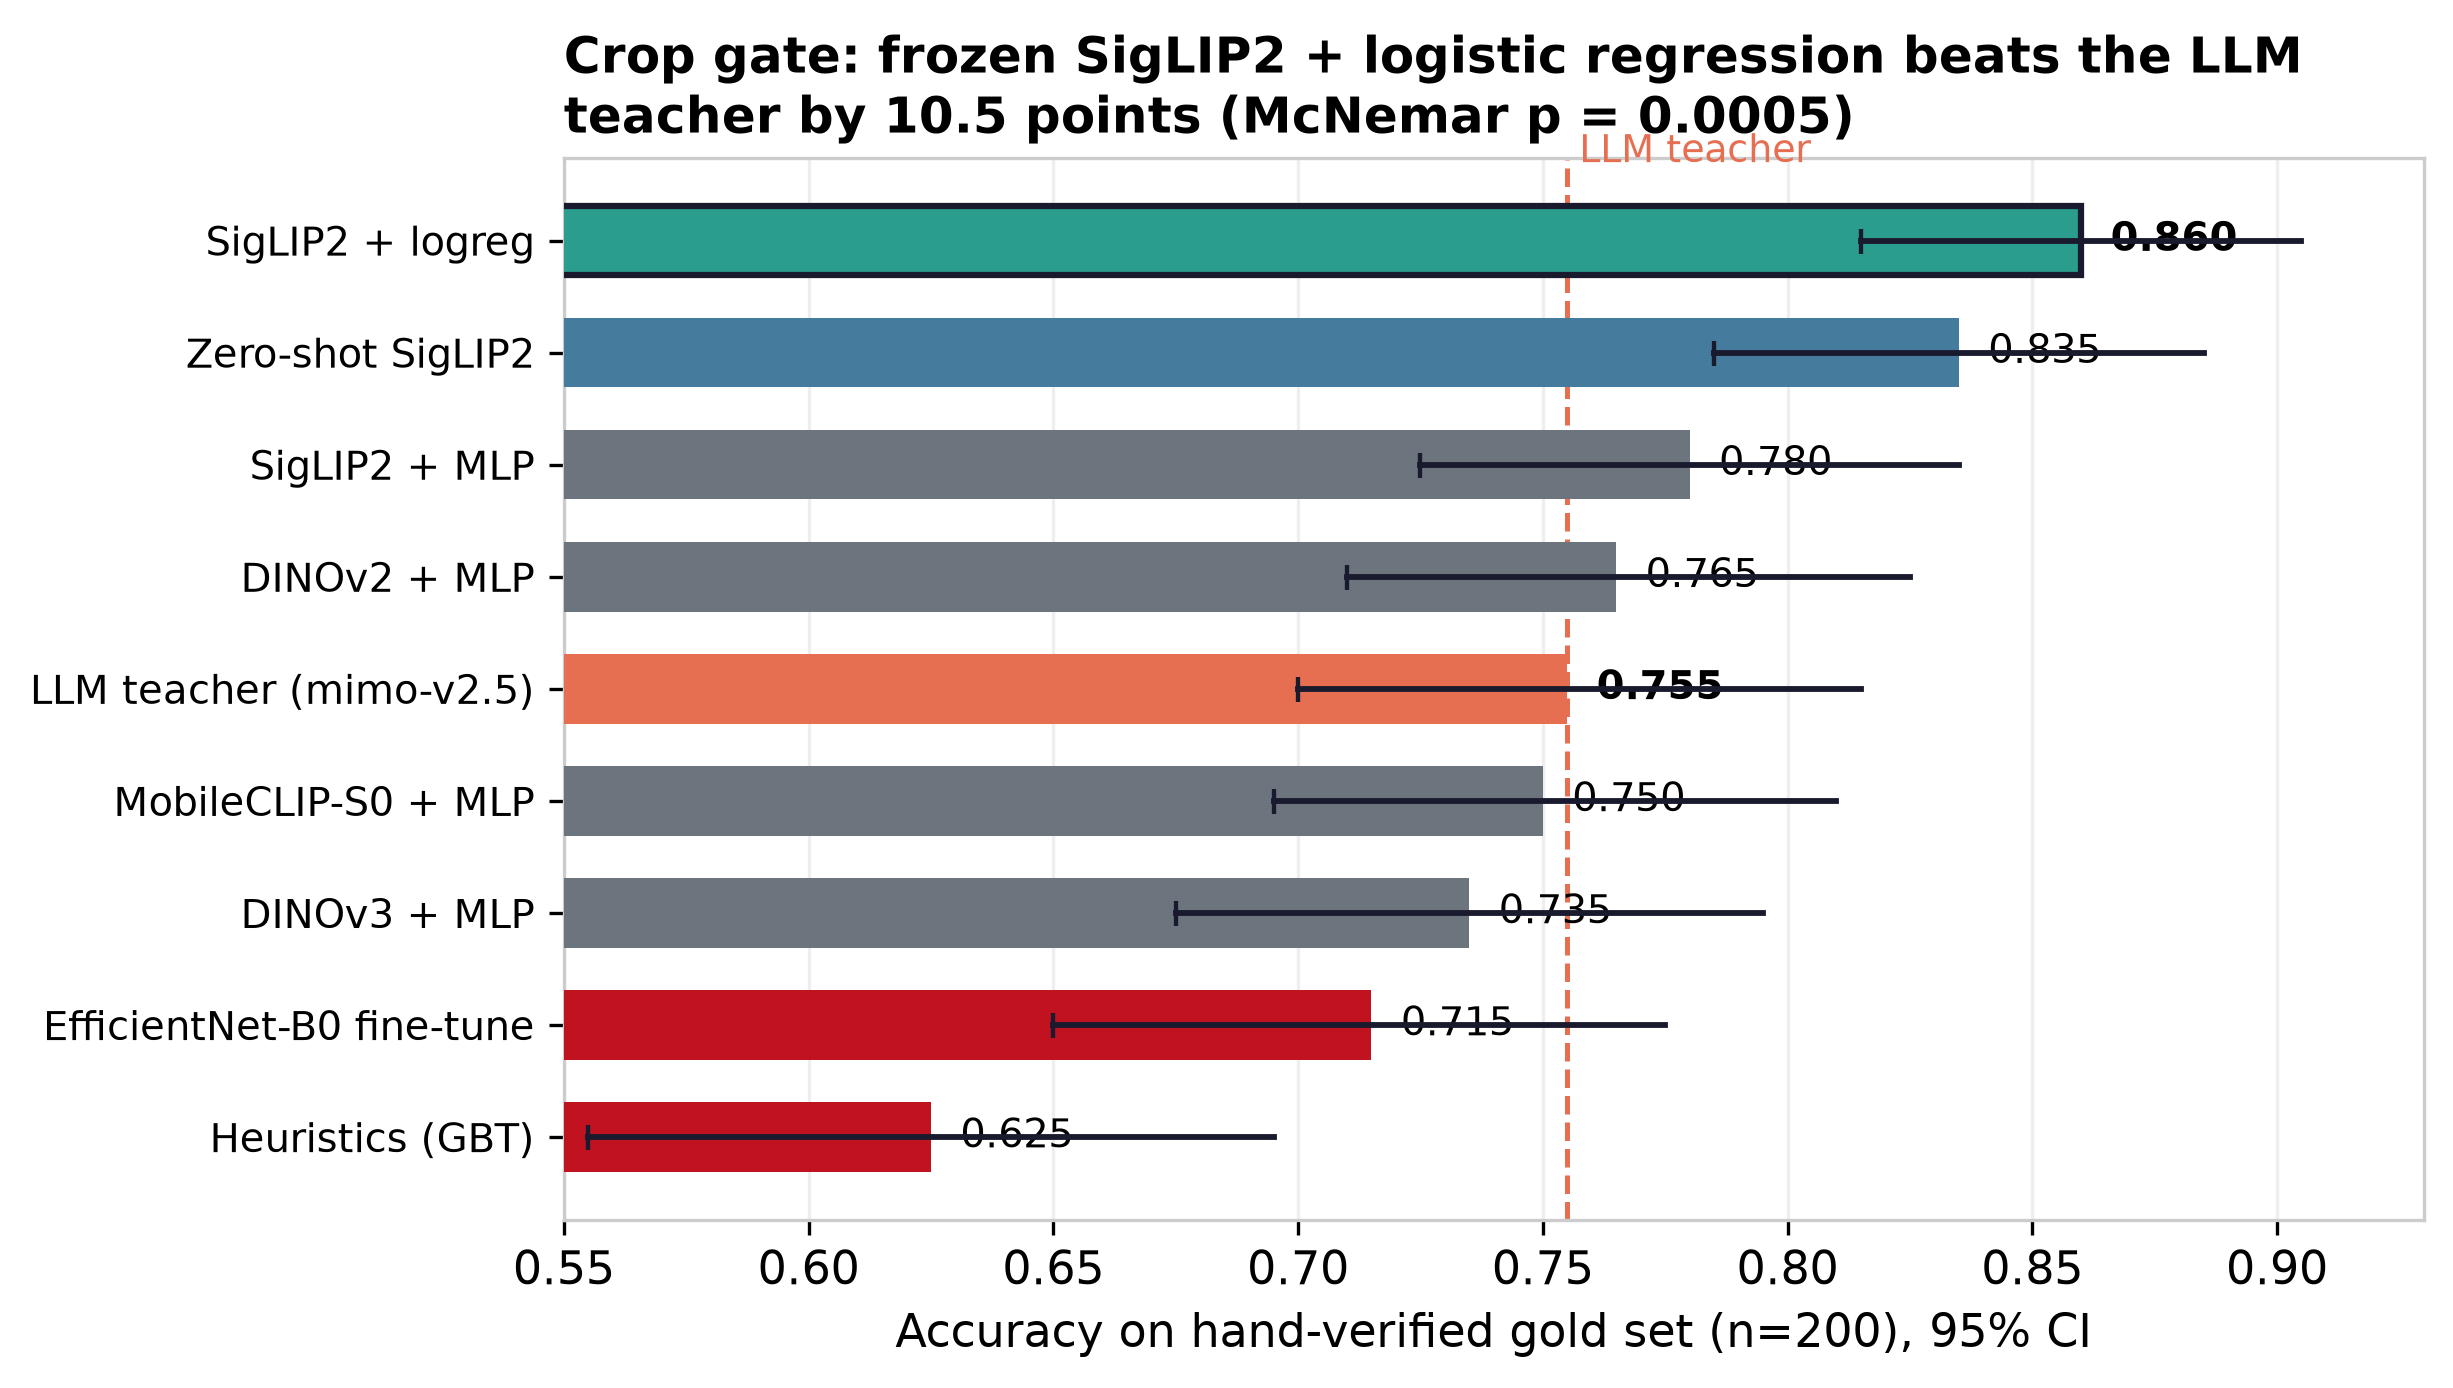
\includegraphics[width=0.92\textwidth]{figures/fig1_gold_leaderboard.png}
\caption{The winner beats the LLM teacher by 10.5 points; the gap is
significant (McNemar $p=0.0005$).}
\label{fig:leaderboard}
\end{figure}

\paragraph{Three findings.}
(1) A frozen SigLIP2 backbone with a logistic-regression head beats the LLM
teacher by 10.5 points, with McNemar $p=0.0005$ (27 cases it fixes vs.\ 6 it
breaks). (2) \emph{Simplicity wins under label noise:} the models that topped
silver-validation --- MLP heads and the fine-tune --- \emph{fell} on gold because
they had the capacity to memorize the teacher's $\sim$25\% wrong labels; the
un-overfittable models generalized (Figure~\ref{fig:flip}). (3) Zero-shot,
with no training at all, also beats the teacher and is statistically tied with
the trained probe (McNemar $p=0.38$).

\begin{figure}[H]\centering
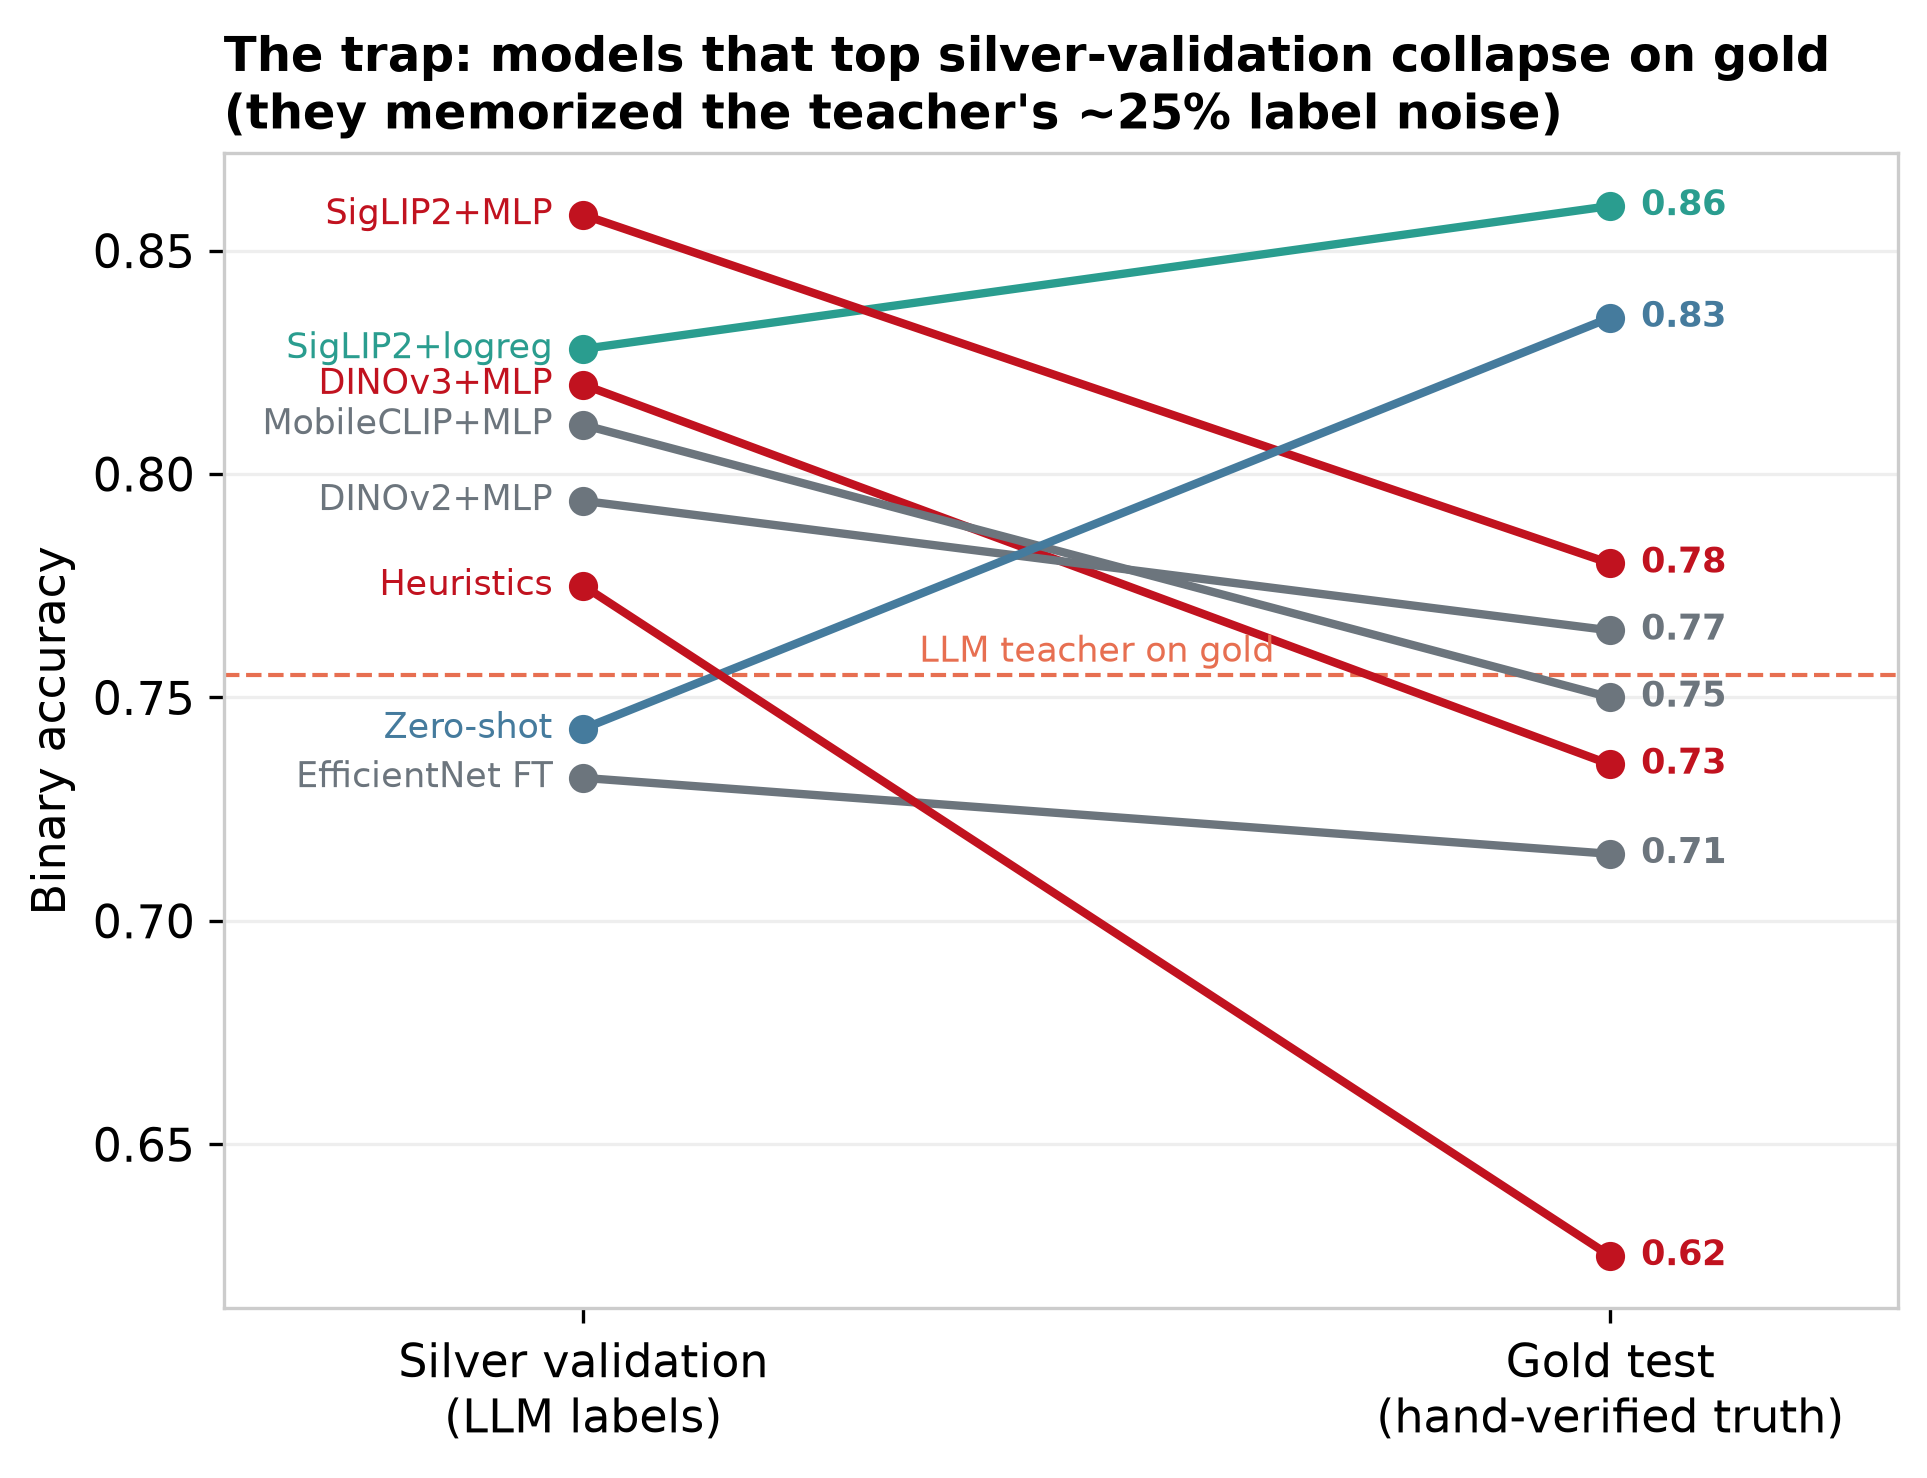
\includegraphics[width=0.7\textwidth]{figures/fig2_silver_vs_gold.png}
\caption{The trap. Ranking on silver validation (LLM labels) selects the model
that generalizes \emph{worst} to gold truth.}
\label{fig:flip}
\end{figure}

\paragraph{Page gate --- a negative result.}
An off-the-shelf DocLayout-YOLO page gate scored 61.7\% on gold (precision
0.44) and ran at 0.2 pages/s: it detects \emph{figures} but cannot separate a
diagram from a plot or photo. The correct page gate reuses the crop
classifier: extract figure regions, classify each, mark the page positive iff
any crop is a diagram.

\paragraph{Speed.}
Table~\ref{tab:speed} and Figure~\ref{fig:speed} give measured latency on an
Apple-Silicon MacBook. The winning gate runs at $\sim$52\,ms/crop on GPU
($\sim$125\,ms CPU), $\sim$100--300$\times$ faster than the LLM per decision,
free and offline.

\begin{table}[H]\centering
\caption{Measured single-image latency (load $\to$ embed $\to$ classify).}
\label{tab:speed}
\begin{tabular}{lcccc}
\toprule
Component & MPS p50 & CPU p50 & Peak RAM & Gold acc \\
\midrule
Heuristic filter & 5.3\,ms & 5.3\,ms & 206\,MB & 0.625 \\
MobileCLIP-S0 + logreg & 20.0\,ms & 168\,ms & 962\,MB & 0.750 \\
EfficientNet-B0 & 27.8\,ms & 529\,ms & 799\,MB & 0.715 \\
\textbf{SigLIP2 + logreg} & \textbf{51.8\,ms} & 125\,ms & 1.0\,GB & \textbf{0.860} \\
DocLayout-YOLO (page) & --- & $\sim$5000\,ms & --- & 0.617 \\
\textcolor{teach}{LLM gate (production)} & --- & 4000--17000\,ms & --- & 0.755 \\
\bottomrule
\end{tabular}
\end{table}

\begin{figure}[H]\centering
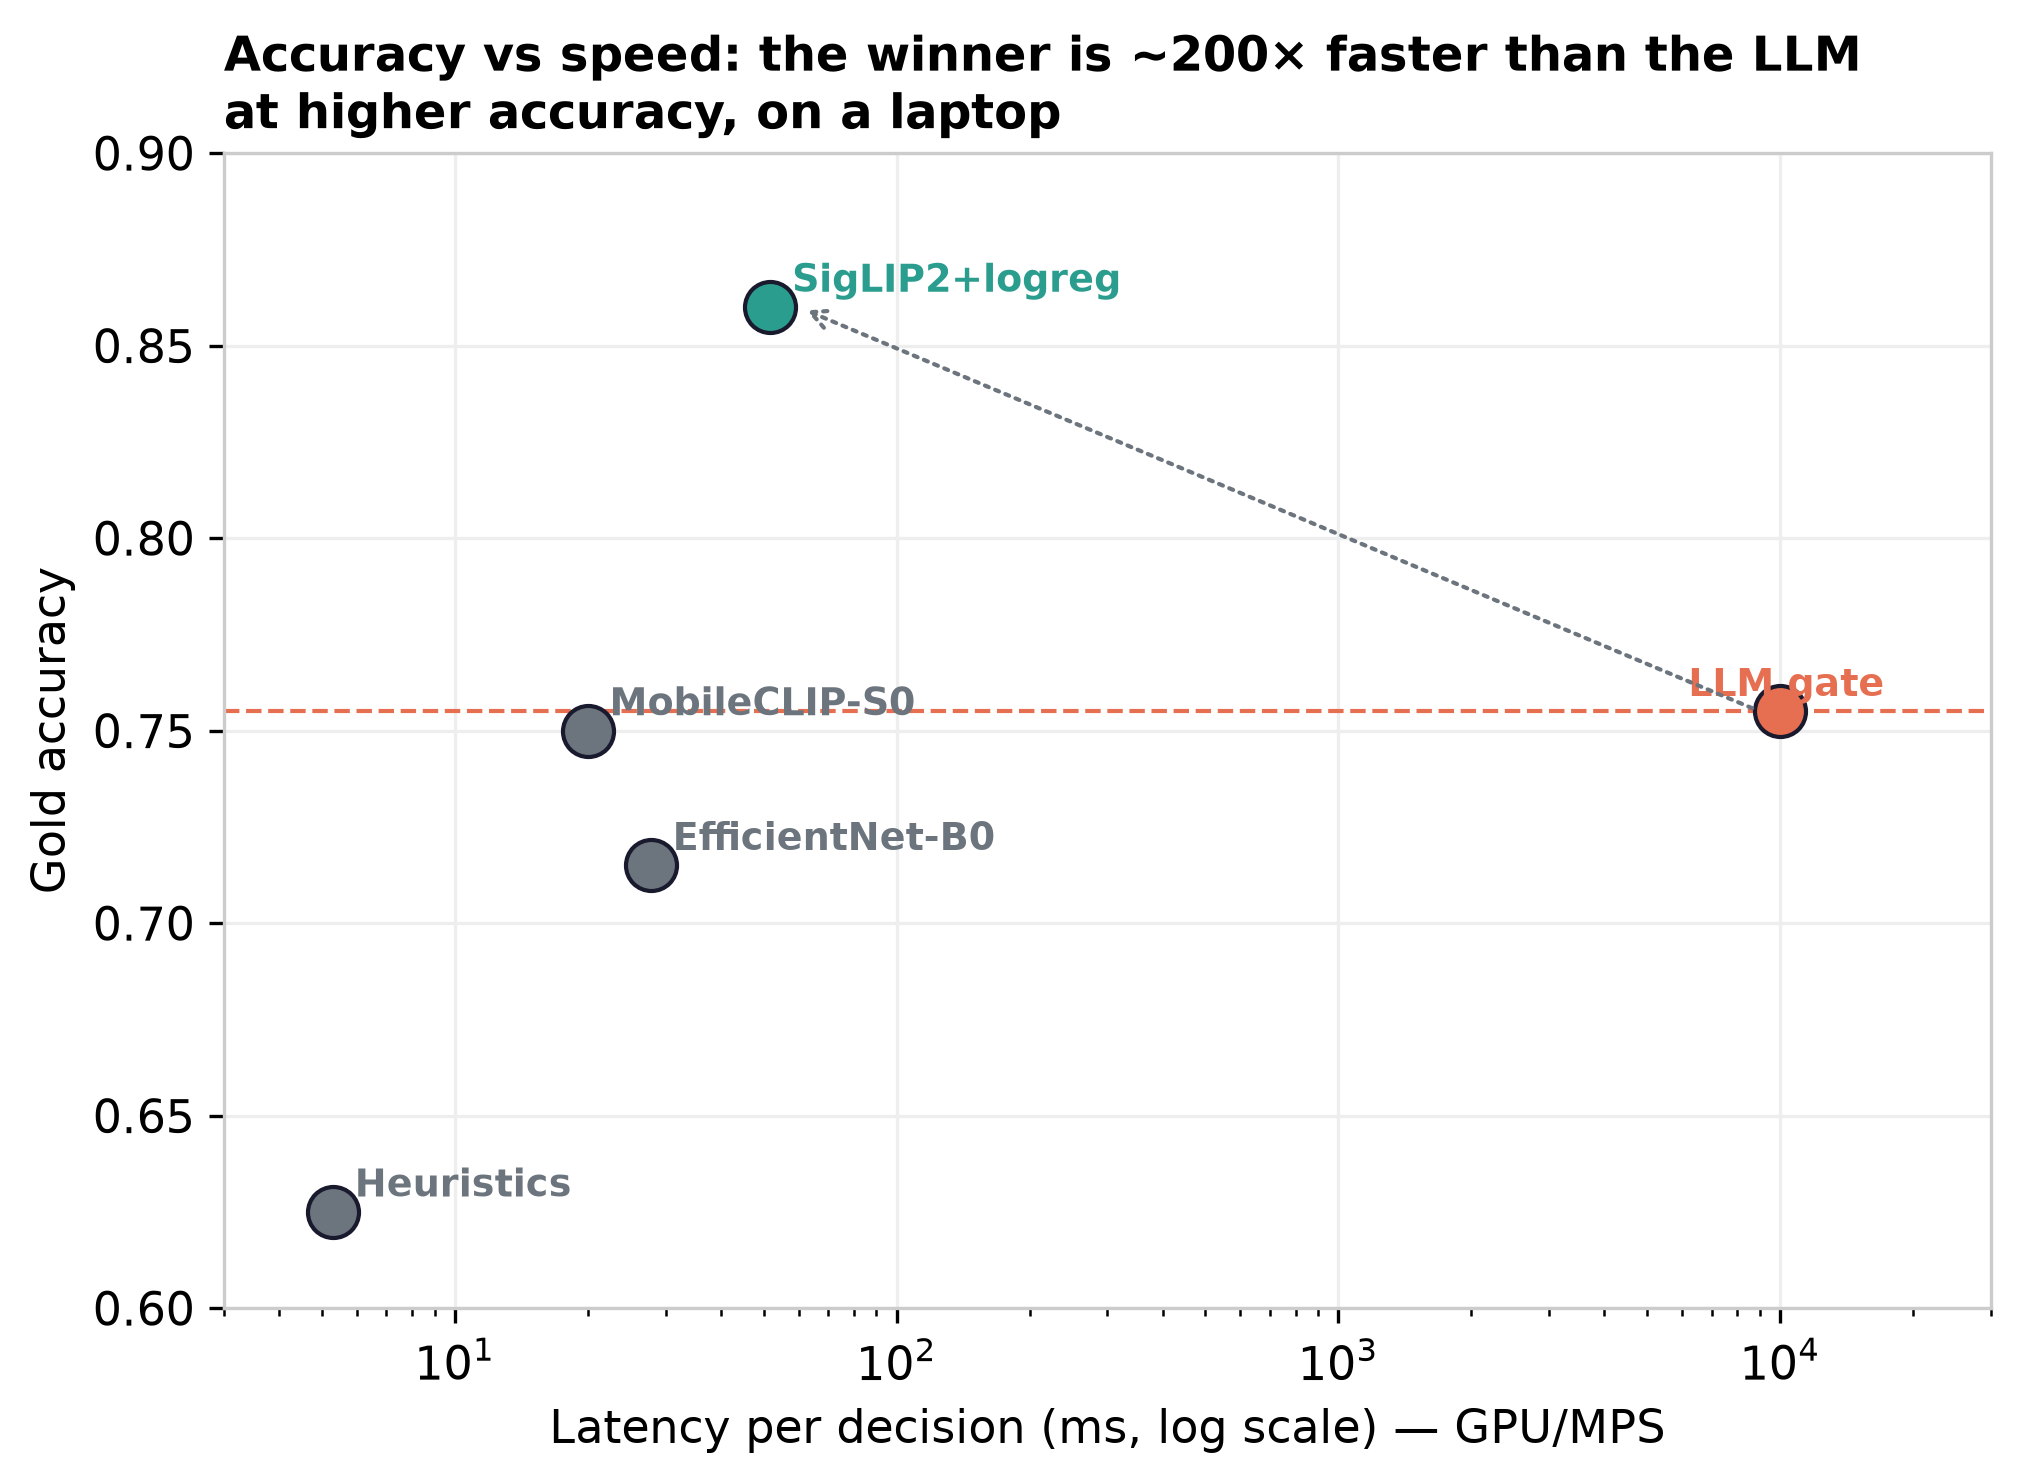
\includegraphics[width=0.82\textwidth]{figures/fig3_speed_accuracy.png}
\caption{Accuracy vs.\ latency. The winner sits top-left; the LLM is two orders
of magnitude slower at lower accuracy.}
\label{fig:speed}
\end{figure}

\paragraph{Does removing the label noise help?}
No (Figure~\ref{fig:ablation}). Confident-learning removal of the estimated
noisiest 4--22\% of training labels left the noise-robust winner flat-to-down
(86.0\%$\to$83--85\%) and only let the overfitting MLP catch up, never past the
simple baseline. Self-cleaning removes information; it cannot add it. Beating
86\% requires independent relabeling or more data, not noise subtraction.

\begin{figure}[H]\centering
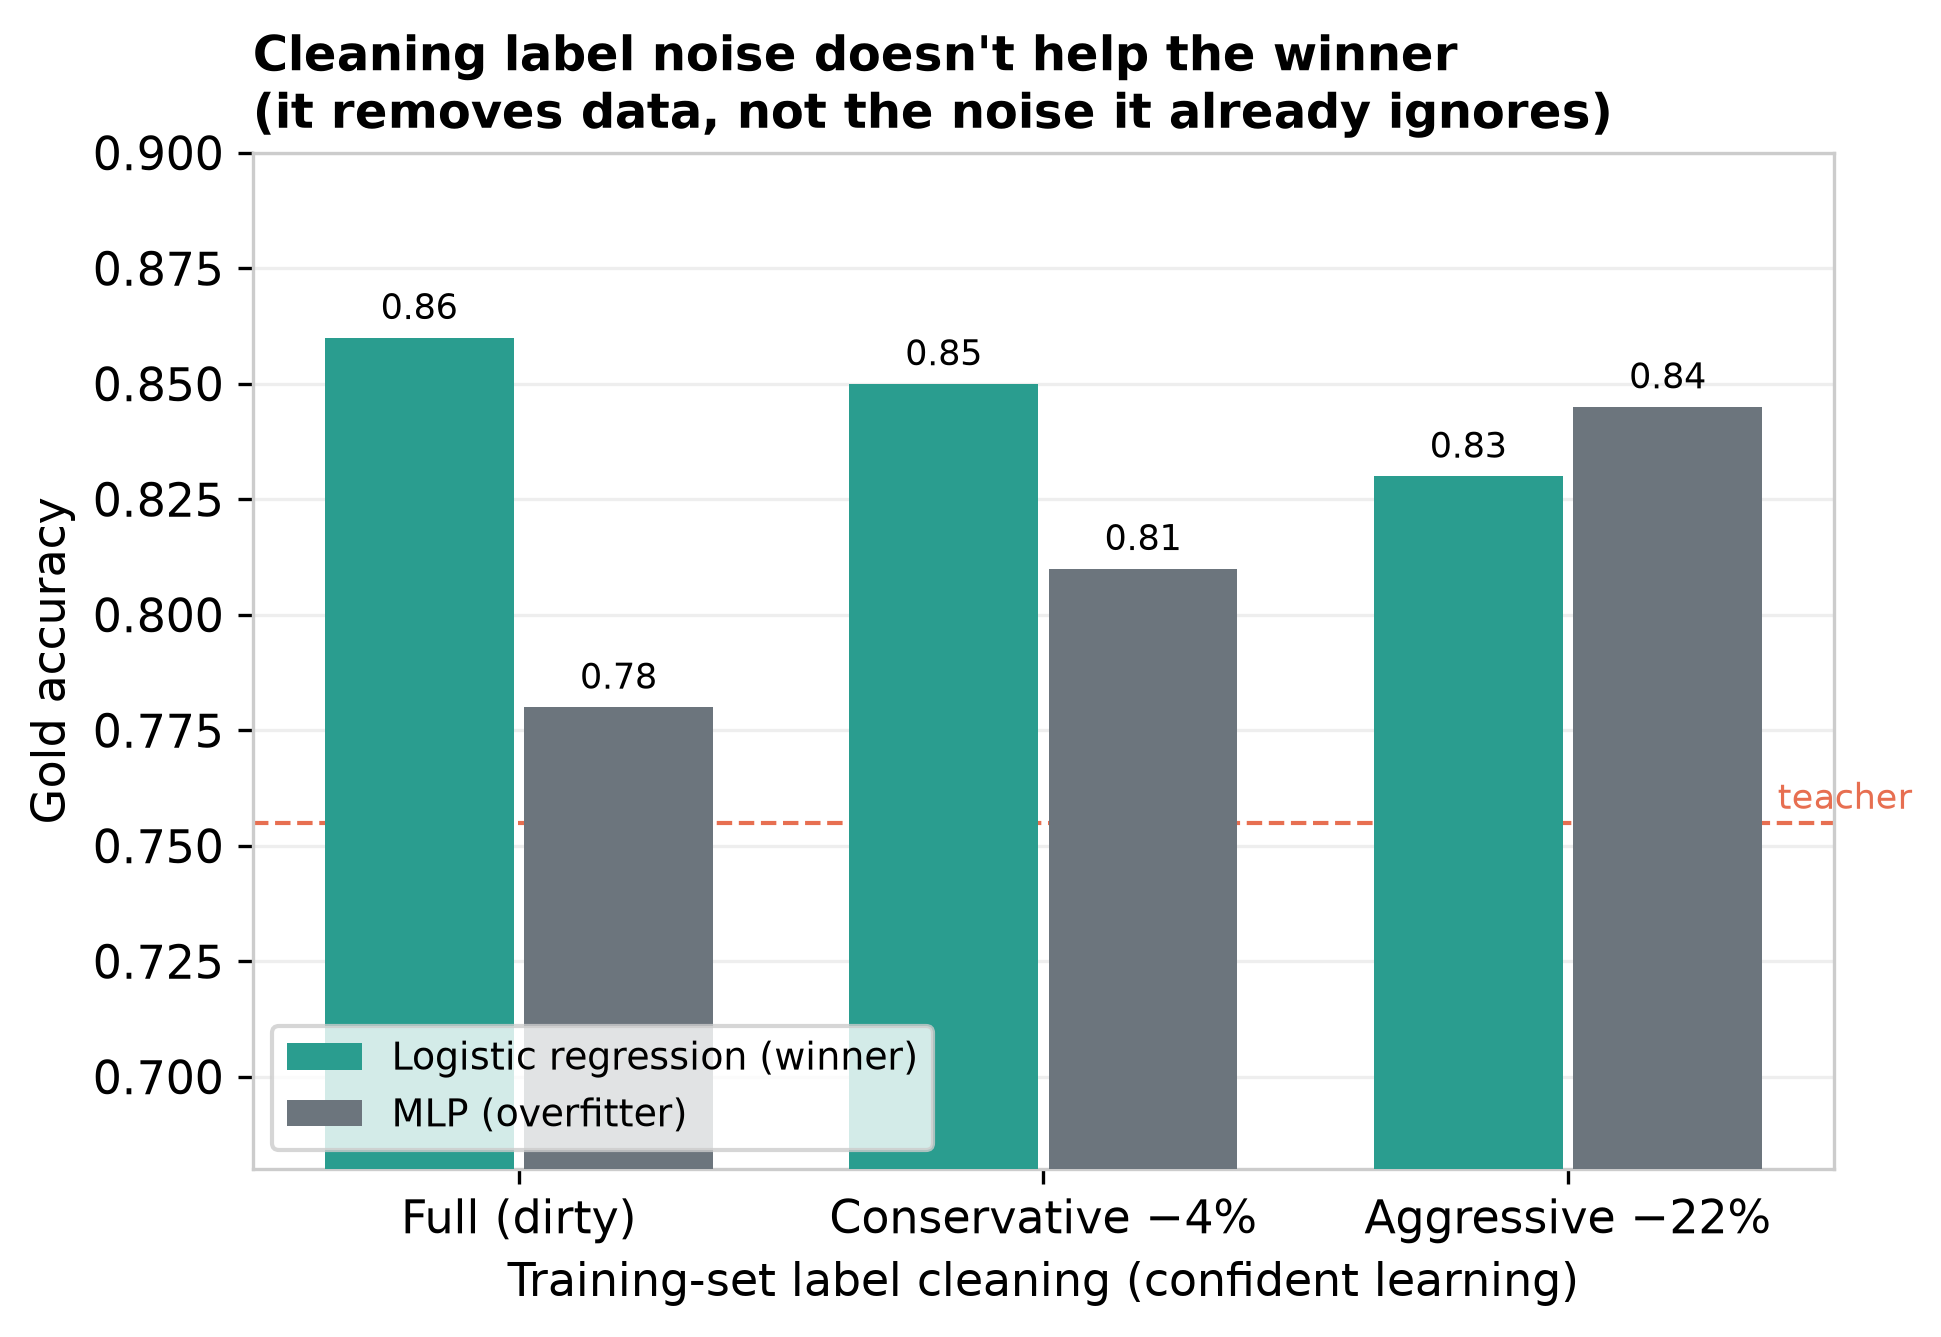
\includegraphics[width=0.62\textwidth]{figures/fig5_ablation.png}
\caption{Label cleaning does not help the winner.}
\label{fig:ablation}
\end{figure}

\section{Production decision}
\textbf{Replace both LLM classification gates with the frozen SigLIP2 +
logistic-regression probe.} It is more accurate than the LLM (significantly
so), $\sim$100--300$\times$ faster, free, offline, and deterministic. Operating
threshold 0.55 gives 95.8\% accept-precision at full coverage; zero-shot
SigLIP2 is the zero-labeled-data fallback, MobileCLIP-S0 (20\,ms) the
low-latency option. Do not fine-tune and do not use an MLP head at this data
scale. The LLM is retained only for \emph{writing} diagram descriptions --- and
only on crops the free gate already accepted. Rollout is shadow-mode first,
then cutover with a 2\% LLM audit stream for drift.

\section{Limitations}
Gold sets are 200 crops / 120 pages, so confidence intervals span a few points
and McNemar ties below $\sim$5 points. The photo class is small (binary is the
reliable metric; 4-class is diagnostic). Robotics is under-represented. Gold
annotators and the teacher are all Claude models; the rubric-anchored blind
protocol and $\kappa$ reporting mitigate but do not eliminate shared-family
bias.

\section*{Artifacts}
Code, data manifests, gold labels, per-experiment JSON, and this paper's
sources are released at \url{https://github.com/adoistic/stem-diagrams}. The
2{,}000-diagram dataset is available at the project site.

\vspace{1em}
\hrule
\vspace{0.6em}
\noindent\small\textbf{About the author.} Adnan Abbasi is the founder of
Thothica.

\end{document}
